\begin{itemize}
  \item dynamic processes involve a set of interacting subprocesses
  \item interactions between subprocesses are sparse
  \item introduces \textbf{local causal models} included from a global causal model by conditioning on a subset of state space
  \item local structures + experience replay to generate counterfactual experiences
  \item locally (during time between interaction) factor dynamics and model subprocesses independently
  \item underlying processes are difficult to model precisely
  \item factored subspaces of observed trajectory pairs are swapped
  \item CoDA is a data-augmentation strategy
  \item use attention to discover local causal structure
  \item improves sample-efficiency in batch-constrained and goal-constrained RL
  \item model time slice $(t, t+1)$ using a structural causal model (SCM)
  \item $\mcal{M}_{t} = \langle V_{t}, U_{t}, \mcal{F} \rangle$ with a DAG $\mcal{G}$
  \item $V_{t}$ is the set of state, action and next states, $U_{t}$ is a set of noise variables and $\mcal{F}$ is the set of structure equations that maps noise $\times$ current state to next state
  \item assume structural minimality allows us to think of edges in $\mcal{G}$ as representing global causal dependence
  \item $P(S_{t+1}^{i}|S_{t}, A_{t}) = P(S_{t+1}^{i}|Pa(S_{t+1}^{i}))$ and $S$ is independent of all nodes that isn't its parent
  \item often exists large subspace ($\mcal{L}^{(j \perp \!\!\! \perp  i)} \subset \mcal{S} \times \mcal{A}$) such that the next state is independent
  \item e.g. two-armed robot, there are many states such that the two arms are too far apart to influence each other
  \item consider a \textit{local causal model} ($\mcal{M}_{t}^{\mcal{L}^{(j \perp \!\!\! \perp i)}}$) whose DAG is strictly sparser than the global DAG
  \begin{figure}[h]
    \caption{Different instances of CoDA}
    \centering
    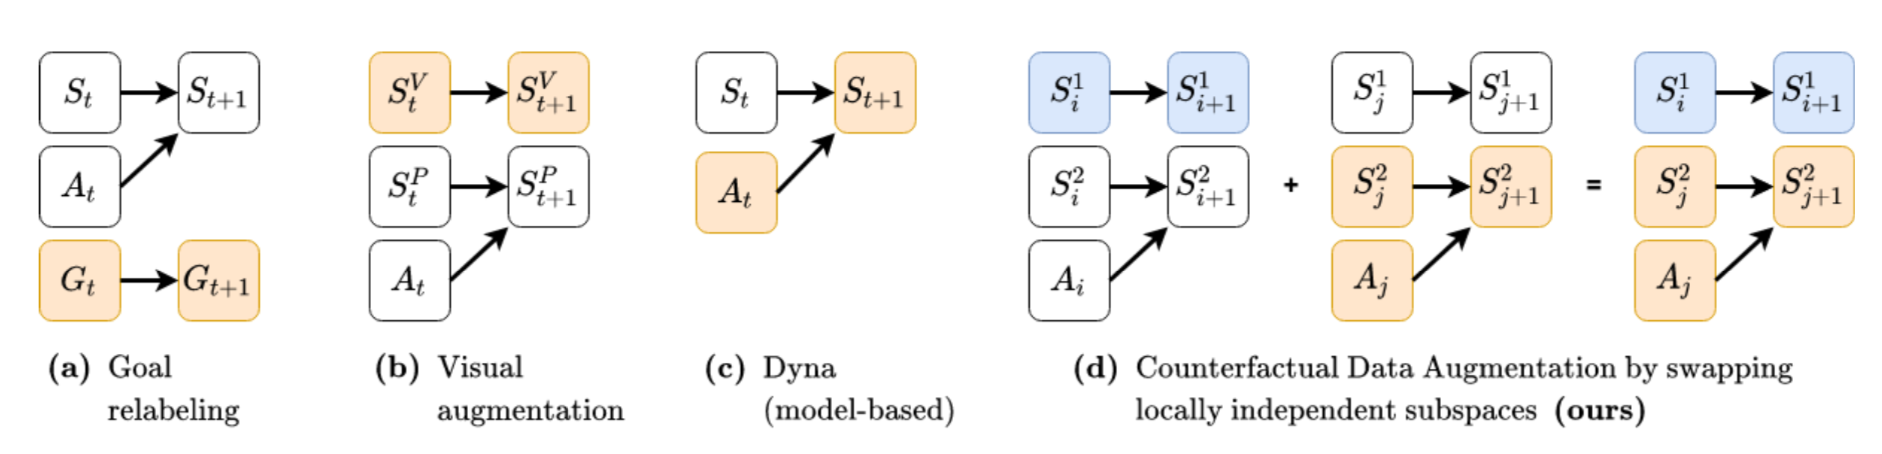
\includegraphics[width=\textwidth]{../../imgs/coda.png}
  \end{figure}
  \item Dyna augments real states with new actions and resamples the next state using a learned dynamics model
  \item can generate an exponential amount of data with CoDA (n independent samples from subspace $\mcal{L}$ whose graph has $m$ connected components $\implies n^{m}$ samples)
  \item CoDA can be used to mix and match data across timesteps
  \begin{figure}[h]
    \caption{CoDA algorithm}
    \centering
    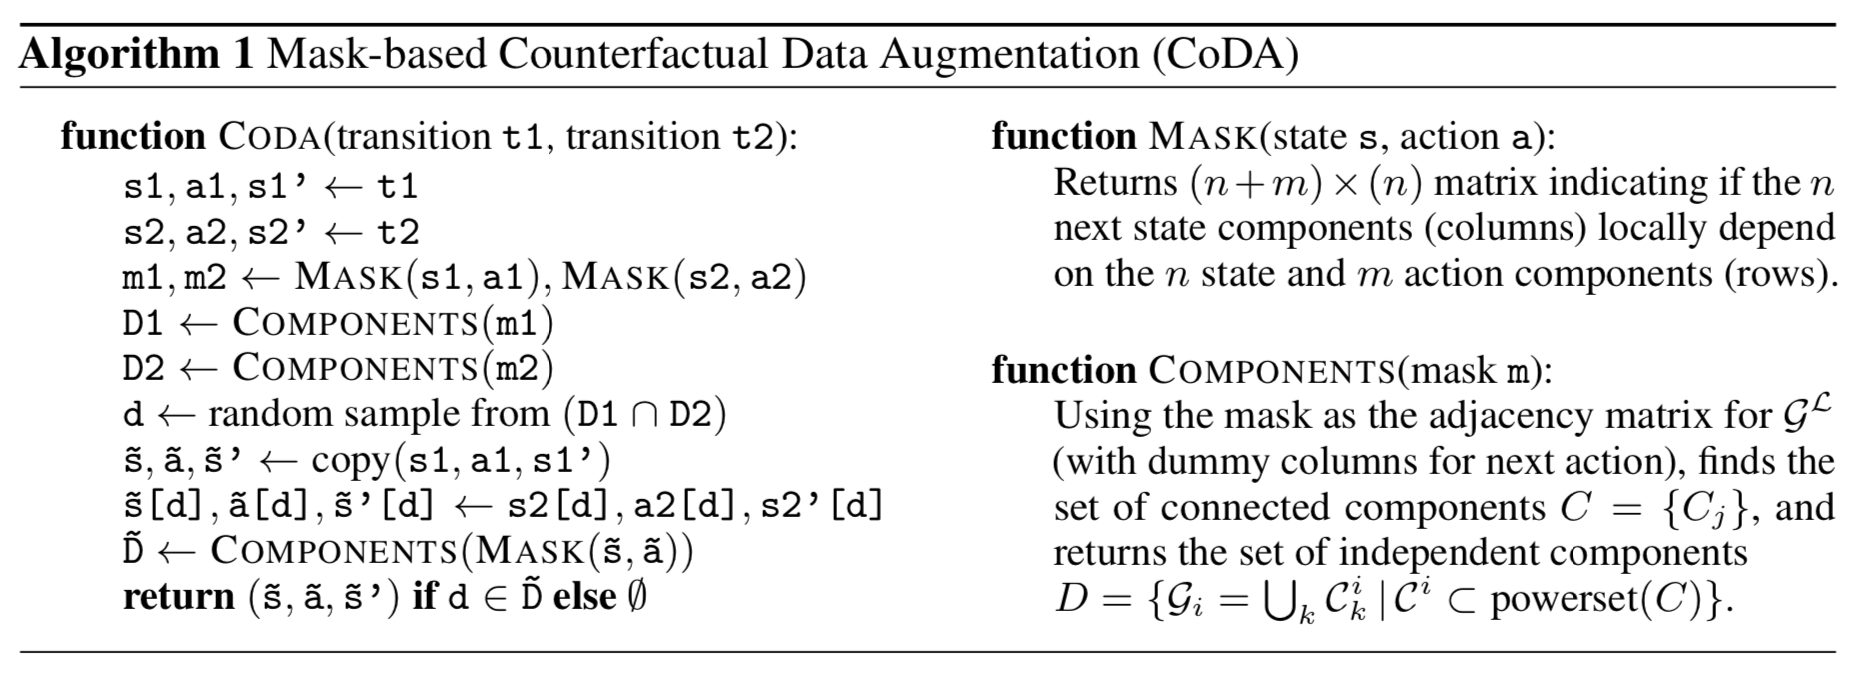
\includegraphics[width=\textwidth]{../../imgs/coda_diagram.png}
  \end{figure}
  \item specify a ratio between observed to counterfactual data to control for selection bias
  \item inferring local fatorization, how to approximate causal model
  \item use a global network mask (MADE) for autoregressive distribution modeling and GraN-DAG for causal discovery
  \item locally conditioned network mask by taking matrix product of locally conditioned layer masks
  \item MLP and single-head set transformer
  \item Inferring local factorization
  \begin{itemize}
    \item SANDy (Sparse Attention Neural Dynamics)
    \item it learns a function or mask that represents the adjacency matrix of the local causal graph
    \item SANDy transformer performs better than MLP in AUC score
    \item SANDy mixture is only sufficient for the simple synthetic MP environments, does not work for Spriteworld
    \item the transformer has stronger inductve bias and more reliably infer local interaction patterns
  \end{itemize}
  \item Some experiment details and notes:
  \begin{itemize}
    \item working with the original TD3 codebase
    \item mask function trained using 42k samples from random policy
    \item increase agent batch size from 256 to 1000, more batch size allows agent to see more of its on-policy data in the face of many off-policy CoDA samples
    \item batch-RL experiment in the Pong environment
    \item trained a transformer to learn a mask function
    \item goal-conditioned RL experiments on OpenAI gym FetchPush environment
    \item these experiments use a hand-coded heuristic designed with domain knowledge
    \item e.g. action is entangled with gripper and gripper + objects are disentangled when they are more than 10cm apart
  \end{itemize}
  \item Other experimental insights:
  \begin{itemize}
    \item tried augmenting the buffer by sampling from a dynamics model similar to model-based RL
    \item good at next-state prediction, but fail to capture collisions and long-term dependencies
  \end{itemize}
\end{itemize}